\chapter{Vybraná pravděpodobnostní rozdělení}

Nejčastěji používané pravděpodobnostní funkce mají přiřazeno jméno. Říkáme tak např., že daná náhodná veličina sleduje normální pravděpodobnostní rozdělení. Stejně jako náhodné veličiny také pravděpodobnostní rozdělení dělíme na spojitá a nespojitá. Následující kapitola je stručným přehledem v praxi nejběžněji používaných pravděpodobnostních rozdělení.

\section{Nespojité pravděpodobnostní rozdělení}

\subsection{Nespojité uniformní rozdělení}

\begin{definition}[Nespojité uniformní rozdělení]
Jestliže má náhodná veličina $X$ pravděpodobnostní funkci
\begin{gather*}
f(x) =
\begin{cases}
\frac{1}{N}~~~\textit{pro}~x = 1,2, ..., N\\
0~~~\textit{v ostatních případech}
\end{cases}\\
=\frac{1}{N}I_{\{1, 2, ..., N\}}(x)
\end{gather*}
kde $N$ je přirozené číslo, říkáme, že tato náhodná veličina sleduje nespojité uniformní rozdělení.
\end{definition}

\begin{figure}[htp]
\centering
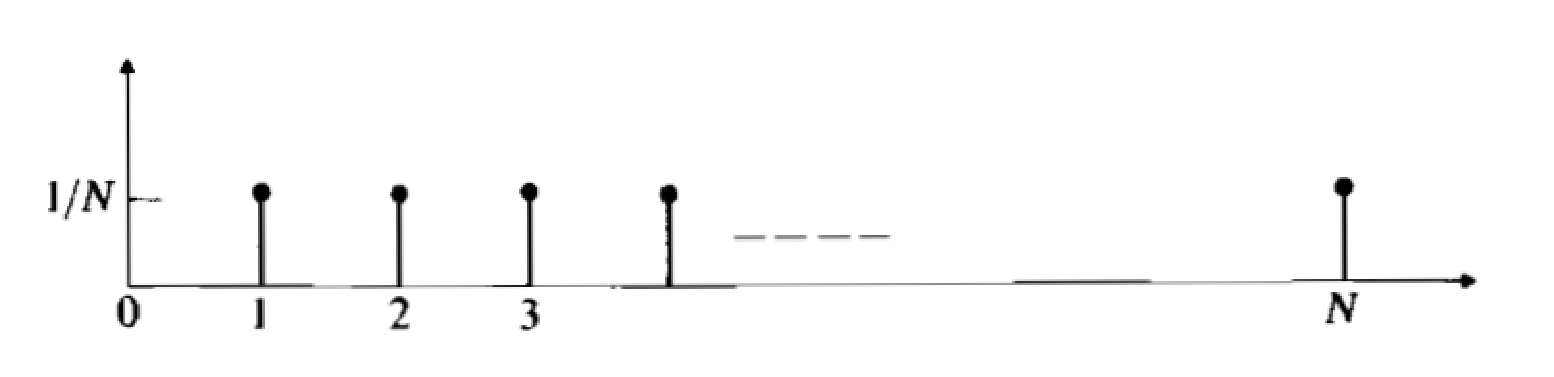
\includegraphics[scale = 0.5]{pictures/discrete_uniform_distribution.eps}
\caption{Pravděpodobnostní funkce nespojitého uniformního rozdělení}
\label{discrete_uniform_distribution}
\end{figure}  

\begin{theorem}
Jestliže náhodná veličina $X$ sleduje nespojité uniformní rozdělení, pak
\begin{gather*}
E[X] = \frac{N+1}{2}\\
D[X] = \frac{N^2 - 1}{12}\\
m(t) = E[e^{tX}] = \sum_{j = 1}^N e^{jt}\frac{1}{N}
\end{gather*}
\end{theorem}

\begin{proof}
\begin{gather*}
E[X] = \sum_{j = 1}^N j \frac{1}{N} = \frac{N+1}{2}\\
D[X] = E[X^2] - E[X]^2 = \sum_{j=1}^N j^2 \frac{1}{N} - \Big( \frac{N+1}{2} \Big)^2\\
= \frac{N(N+1)(2N+1)}{6N} - \frac{(N+1)^2}{4} = \frac{(N+1)(N-1)}{12}\\
E[e^{tX}] = \sum_{j = 1}^N e^{jt} \frac{1}{N}
\end{gather*}
\end{proof}

Někdy je nespojité diskrétní rozdělení definována jako
\begin{equation*}
f(x) = \frac{1}{N+1}I_{\{0,1,...,N\}}(x)
\end{equation*}
V těchto případech je třeba výše uvedené rovnice upravit.

\subsection{Bernoulliho a binomické rozdělení}

\subsubsection{Bernoulliho rozdělení}

\begin{definition}[Bernoulliho rozdělení]
Říkáme, že náhodná veličina $X$ sleduje Bernoulliho rozdělení, jestliže má její pravděpodobnostní rozdělení tvar
\begin{equation*}
f(x) =
\begin{cases}
p^x(1-p)^{1-x}~~~\text{pro}~x = 0, 1\\
0~~~\textit{v ostatních případech}
\end{cases}\\
= p^x(1-p)^{1-x}I_{\{0,1\}}(x)
\end{equation*}
kde $0 \le p \le 1$. Parameter $1-p$ se velmi často označuje jako $q$.
\end{definition}

\begin{figure}[htp]
\centering
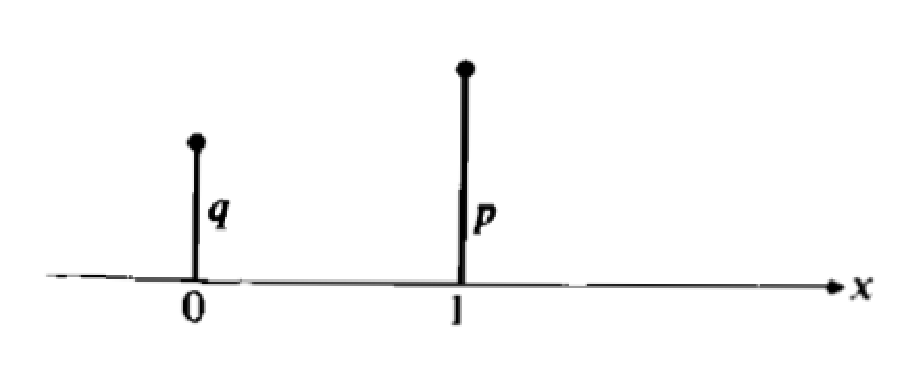
\includegraphics[scale = 0.5]{pictures/bernoulli_distribution.eps}
\caption{Pravděpodobnostní funkce Bernoulliho rozdělení}
\label{bernoulli_distribution}
\end{figure}  

\begin{theorem}
Jestliže náhodná veličina $X$ sleduje Bernoulliho rozdělení, pak
\begin{gather*}
E[X] = p\\
D[X] = pq\\
m(t) = pe^t + q\\
\end{gather*}
\end{theorem}

\begin{proof}
\begin{gather*}
E[X] = 0 \cdot q + 1 \cdot p = p\\
D[X] = E[X^2] - E[X]^2 = 0^2 \cdot q + 1^2 \cdot p - p^2 = pq\\
m(t) = E[e^{tX}] = e^{0 \cdot t} p^0 q^1 + e^{1 \cdot t} p^1 q^0 = q + e^t p
\end{gather*}
\end{proof}

\begin{example}
Uvažujme hod hrací kostkou. Úspěch definujme jako situaci, kdy padne číslo šest a neúspěch, jestliže padne číslo jedna až pět. Odpovídající náhodná veličina má povahu Bernoulliho rozdělení s pravděpodobností úspěchu $p = \frac{1}{6}$.
\end{example}

\subsubsection{Binomické rozdělení}

\begin{definition}[Binomické rozdělení]
Náhodná veličina $X$ sleduje binomické rozdělení, jestliže její pravděpodobnostní funkce je
\begin{equation*}
f(x) = 
\begin{cases}
\binom{n}{x} p^x q^{n-x}~~~\textit{pro}~x=0,1,...,n\\
0~~~\textit{v ostatních případech}
\end{cases}\\
=\binom{n}{x}p^xq^{n-x}I_{\{0,1,...,n\}}(x)
\end{equation*}
kde $0 \le p \le 1$, $n$ je přirozené číslo a $q = 1 - p$.
\end{definition}

\begin{figure}[htp]
\centering
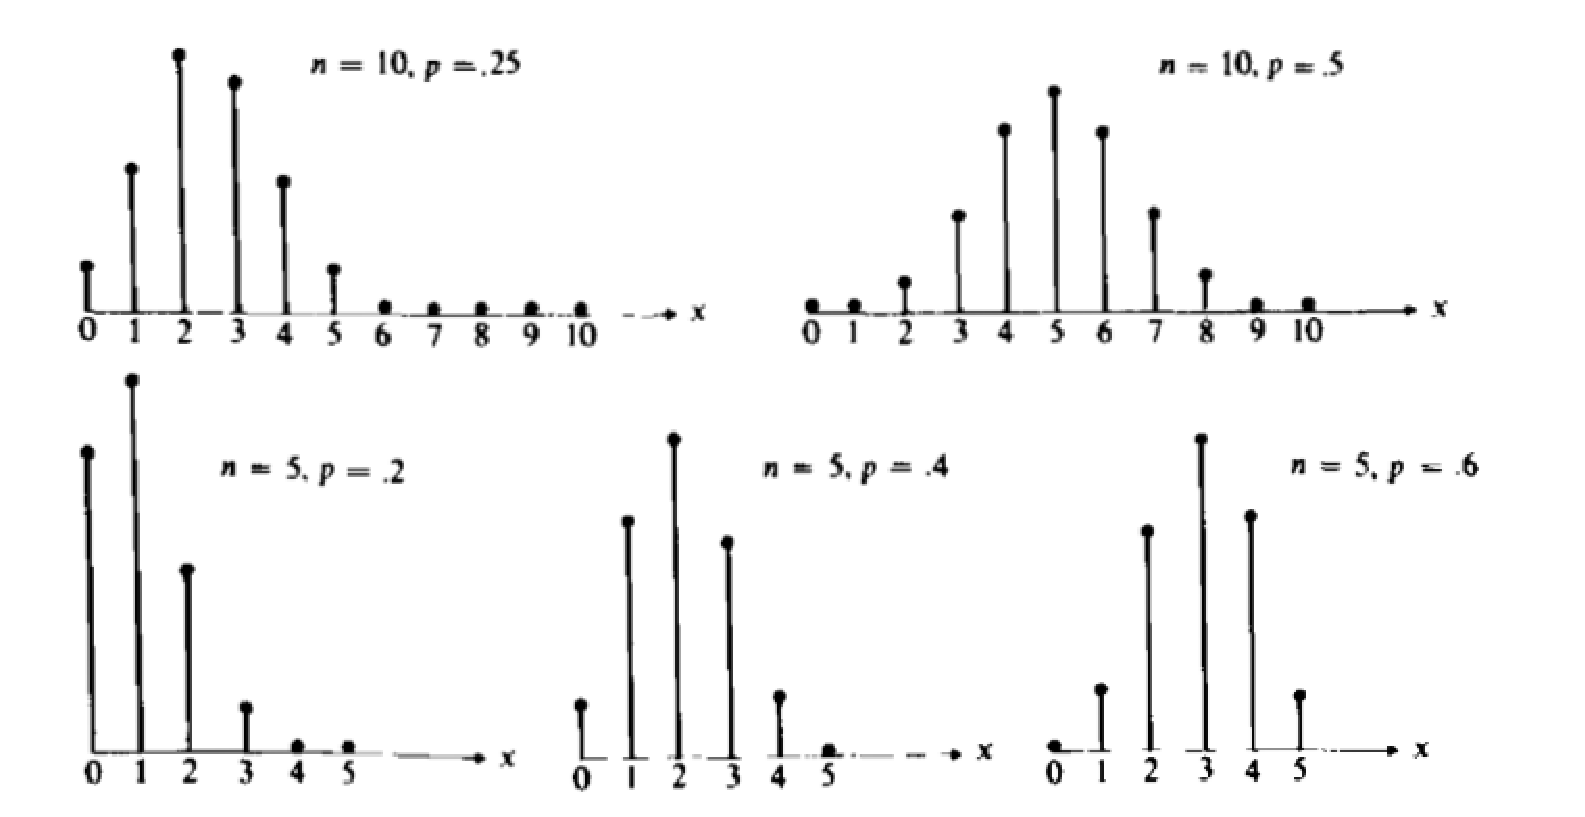
\includegraphics[scale = 0.5]{pictures/binomial_distribution.eps}
\caption{Pravděpodobnostní funkce binomického rozdělení}
\label{binomial_distribution}
\end{figure} 

\begin{theorem}
Jestliže náhodná velčina $X$ sleduje binomické rozdělení, pak
\begin{gather*}
E[X] = np\\
D[X] = npq\\
m(t) = (q + pe^t)^n
\end{gather*}
\end{theorem}

\begin{proof}
\begin{gather*}
m(t) = E[e^{tX}] = \sum_{x=0}^ne^{tx}\binom{n}{x}p^x q^{n-x}=\sum_{x=0}^n \binom{n}{x}(pe^t)^xq^{n-x} = (pe^t + q)^n\\
m'(t) = npe^t(pe^t + q)^{n-1}\\
m''(t) = n(n-1)(pe^t)^2(pe^t + q)^{n-2} + npe^t(pe^t + q)^{n-1}
\end{gather*}
a proto
\begin{gather*}
E[X] =  m'(0) = np\\
D[X] = E[X^2] - E[X]^2 = m''(0) - (np)^2 = n(n-1)p^2 + np - (np)^2 = np(1-p)
\end{gather*}
\end{proof}
Je-li $n=1$ zredukuje se binomické na Bernoulliho rozdělení.
\begin{example}
Uvažujme hod pěti hracími kostkami. Jaká je pravděpodobnost, že číslo šest padne právě dvakrát?

Jedním z možných řešení je situace, kdy v prvních třech hodech padlo číslo jedna až pět a číslo šest padlo v posledních dvou hodech. Pravděpodobnost této kombinace je $\big(\frac{5}{6}\big)^3\big(\frac{1}{6}\big)^2$. Vzhledem k tomu, že však nezáleží na pořadí hodů, existuje $\binom{5}{2}$ takovýchto řešení. Výsledná pravděpodobnost je tak rovna
\begin{equation*}
\binom{5}{2}\Big(\frac{5}{6}\Big)^3\Big(\frac{1}{6}\Big)^2 = 0.1608
\end{equation*} 
\end{example}

Jak vyplývá z následující věty, pravděpodobnostní funkce binomického rozdělení nejprve monotónně roste a následně monotónně klesá.
\begin{theorem}
Nechť náhodná veličina $X$ sleduje binomické rozdělení. Pak
\begin{enumerate}
\item $f(x-1) < f(x)$ jestliže $x < (n + 1)p$,
\item $f(x-1) > f(x)$ jestliže $x > (n + 1)p$ a
\item $f(x-1) = f(x)$ jestliže $x = (n + 1)p$ a $(n + 1)p$ je celé číslo pro $x = 1, 2, ...,n$.
\end{enumerate}
\end{theorem}

\begin{proof}
\begin{equation*}
\frac{f(x)}{f(x-1)} = \frac{n - x + 1}{x} \frac{p}{q} = 1 + \frac{(n + 1)p - x}{xq}
\end{equation*}
Výše uvedené je
\begin{enumerate}
\item větší než 1, jestliže $x < (n + 1)x$,
\item menší než 1, jestliže $x > (n + 1)x$ a
\item rovno 1, jestliže $x = (n + 1)x$.
\end{enumerate}
\end{proof}

\subsection{Hypergeometrické rozdělení}

\begin{definition}[Hypergeometrické rozdělení]
Jestliže náhodná veličina $X$ sleduje hypergeometrické rozdělení, pak je její pravděpodobnostní funkce definována jako
\begin{gather*}
f(x) =
\begin{cases}
\frac{\binom{K}{x}\binom{M-K}{n-x}}{\binom{M}{n}}~~~\textit{pro}~x = 0,1,...,n\\
0~~~\textit{v ostatních případech}
\end{cases}\\
= \frac{\binom{K}{x}\binom{M-K}{n-x}}{\binom{M}{n}}I_{\{0,1,...,n\}}(x)
\end{gather*}
kde $M > 0$, $0 \le K \le M$, $0 < n \le M$. 
\end{definition}

\begin{figure}[htp]
\centering
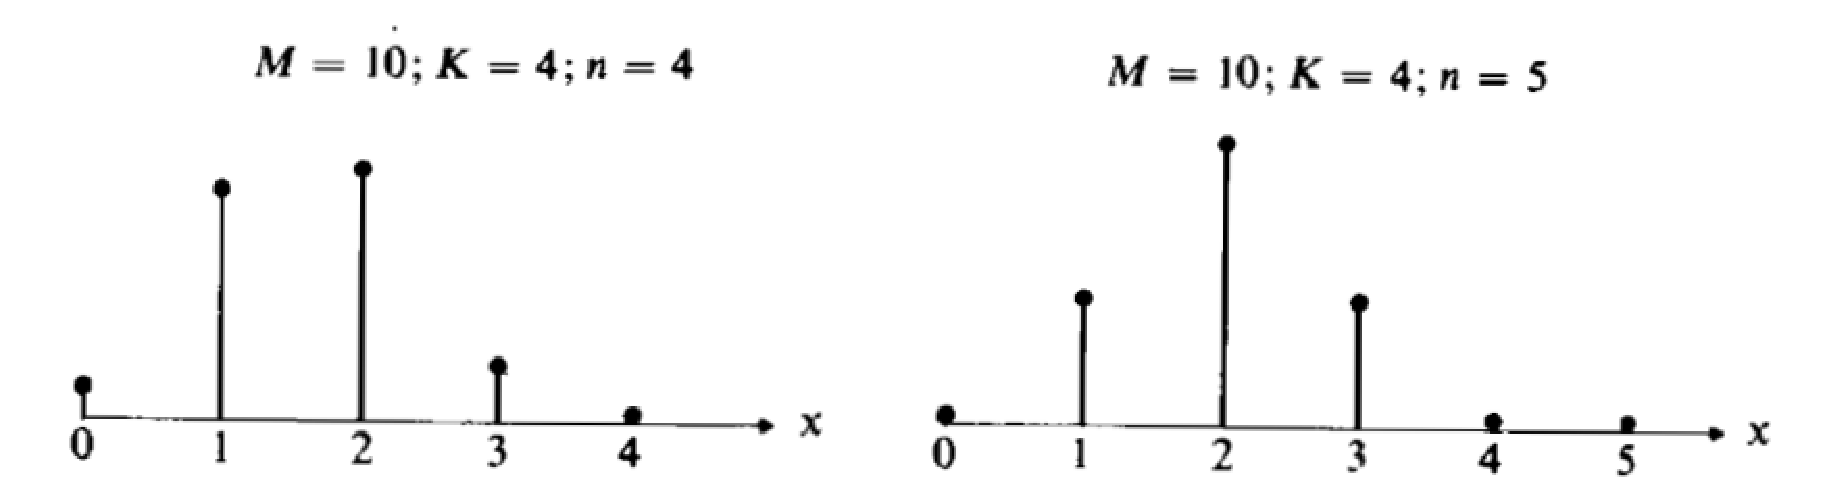
\includegraphics[scale = 0.5]{pictures/hypergeometric_distribution.eps}
\caption{Pravděpodobnostní funkce hypergeometrického rozdělení}
\label{hypergeometric_distribution}
\end{figure}

\begin{theorem}
Jestliže náhodná veličina $X$ sleduje hypergeometrické rozdělení, pak
\begin{gather*}
E[X] = n \frac{K}{M}\\
D[X] = n \frac{K}{M} \frac{M-K}{M}\frac{M-n}{M-1}
\end{gather*}
\end{theorem}

\begin{proof}
\begin{gather*}
E[X] = \sum_{x=0}^n x \frac{\binom{K}{x}\binom{M - K}{n-x}}{\binom{M}{n}} = n \frac{K}{M}\sum_{x=1}^n \frac{\binom{K-1}{x-1}\binom{M-K}{n-x}}{\binom{M-1}{n-1}}\\
= n \frac{K}{M} \sum_{y=0}^{n-1} \frac{\binom{K-1}{y}\binom{M-1-K+1}{n-1-y}}{\binom{M-1}{n-1}}=n \frac{K}{M}
\end{gather*}
s využitím vztahů $\binom{a}{b} = \frac{a}{b}\binom{a-1}{b-1}$ a $\sum_{i=0}^m \binom{a}{i}\binom{b}{m-i} = \binom{a + b}{m}$. Dále platí
\begin{gather*}
E[X(X-1)] = \sum_{x = 0}^n x(x-1)\frac{\binom{K}{x} \binom{M-K}{n-x}}{\binom{M}{n}} = n(n-1)\frac{K(K-1)}{M(M-1)}\sum_{x=2}^n \frac{\binom{K-2}{x-2}\binom{M-K}{n-x}}{\frac{M-2}{n-2}}\\
= n(n-1)\frac{K(K-1)}{M(M-1)}\sum_{y=0}^{n-2} \frac{\binom{K-2}{y}\binom{M-2-K+2}{n-2-y}}{\binom{M-2}{n-2}} = n (n-1) \frac{K(K-1)}{M(M-1)}
\end{gather*}
A proto
\begin{gather*}
D[X] = E[X^2] - E[X]^2 = E[X(X-1)] + E[X] - E[X]^2\\
= n(n-1)\frac{K(K-1)}{M(M-1)} + n \frac{K}{M}-n^2 \frac{K^2}{M^2} = n \frac{K}{M}\Big((n-1)\frac{K-1}{M-1} + 1 - \frac{nK}{M} \Big)\\
= \frac{nK}{M}\Big(\frac{(M-K)(M-n)}{M(M-1)} \Big)
\end{gather*}
\end{proof}

Jestliže dosadíme $\frac{K}{M} = p$, pak se střední hodnota hypergeometrického rozdělení shoduje se střední hodnotou binomického rozdělení a rozptyl hypergeometrického rozdělení je $\frac{M-n}{M-1}$ krát rozptyl binomického rozdělení.

\begin{example}
Nechť $X$ označuje počet vadných výrobků ve vzorku velikosti $n$, který byl získán výběrem bez vracení z populace $M$ výrobků, z nichž celkem $K$ bylo vadných. Takto definovaná náhodná veličina sleduje hypergeometrické rozdělení.
\end{example}

\subsection{Poissonovo rozdělení}

\begin{definition}[Poissonovo rozdělení]
Náhodná veličina $X$ sleduje Poissonovo rozdělení, jestliže její pravděpodobnostní funkce je definována jako
\begin{gather*}
f(x) =
\begin{cases}
\frac{e^{-\lambda}\lambda^x}{x!}~~~\textit{pro}~x = 0,1,2, ...\\
0 ~~~\textit{v ostatních případech}
\end{cases}\\
= \frac{e^{-\lambda}\lambda^x}{x!}I_{\{0,1,2, ...\}}(x)
\end{gather*}
kde $\lambda > 0$.
\end{definition}

\begin{figure}[htp]
\centering
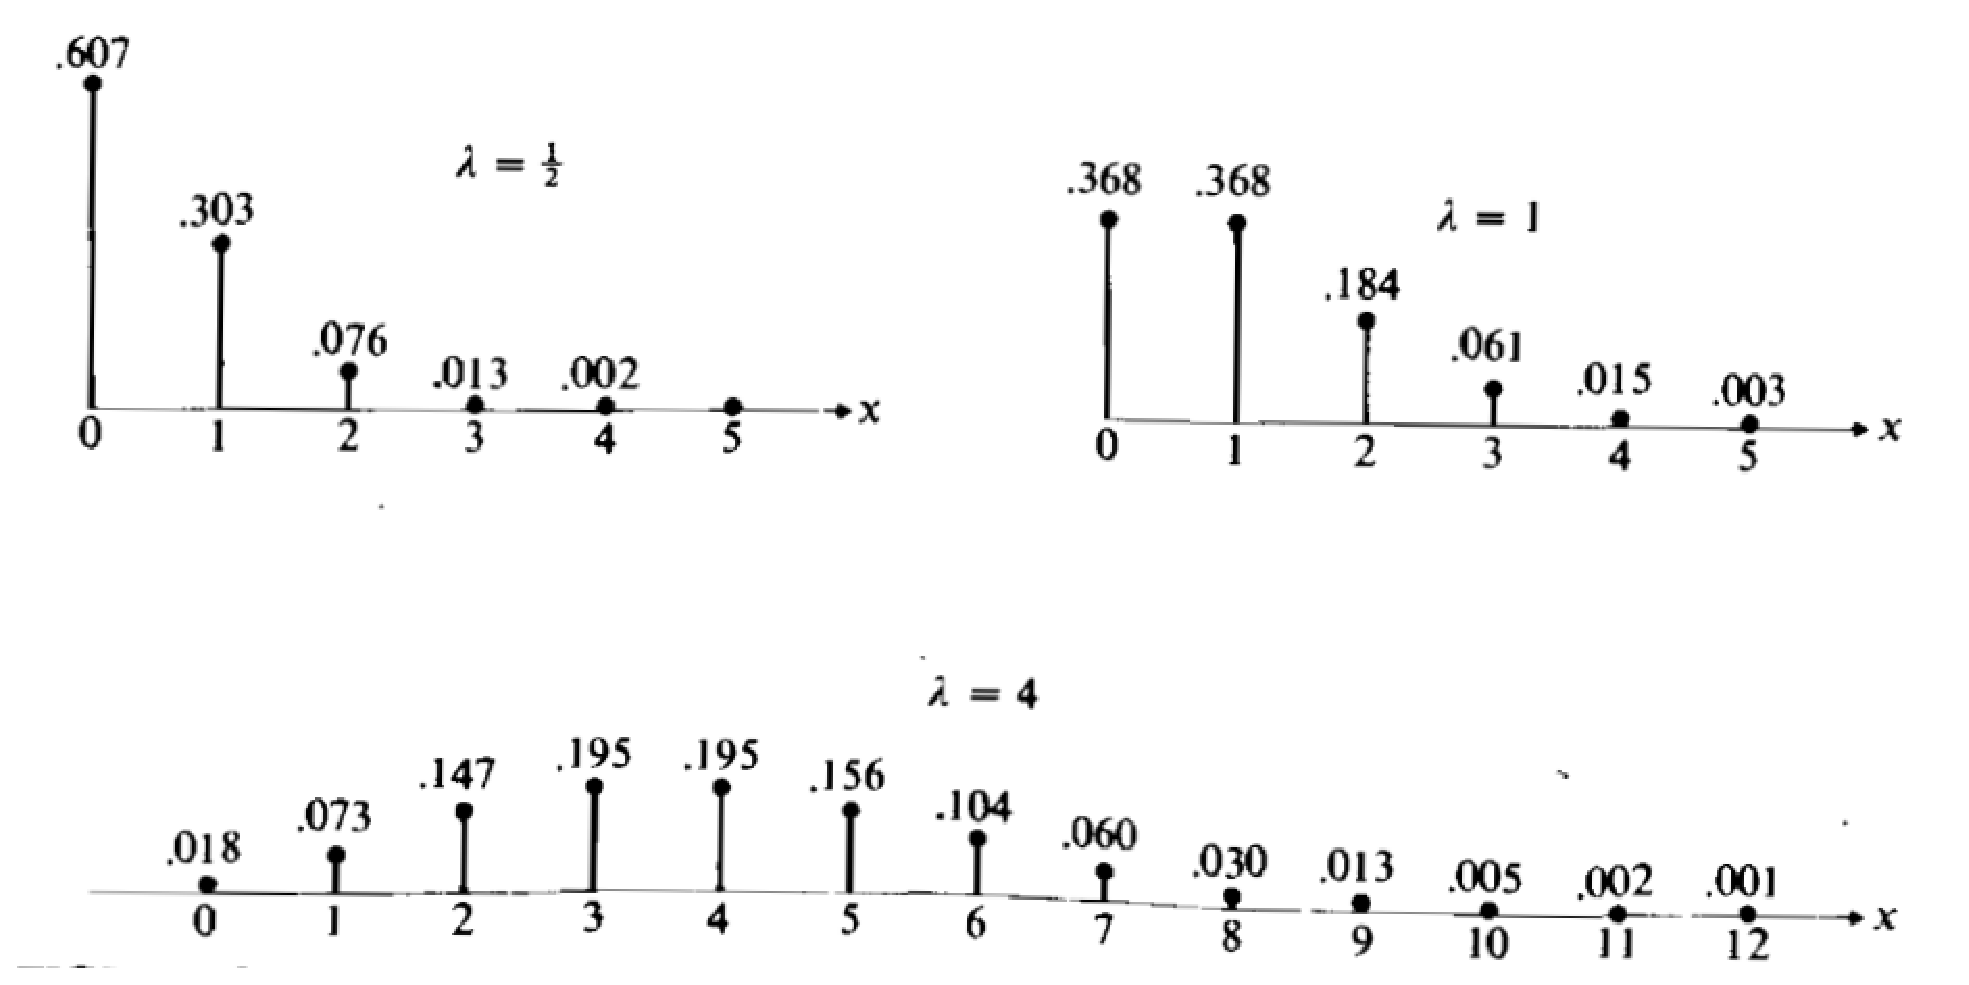
\includegraphics[scale = 0.35]{pictures/poisson_distribution.eps}
\caption{Pravděpodobnostní funkce Poissonova rozdělení}
\label{poisson_distribution}
\end{figure}

\begin{theorem}
Nechť náhodná veličina $X$ sleduje Poissonovo rozdělení. Pak
\begin{gather*}
E[X] = \lambda\\
D[X] = \lambda\\
m(t) = e^{\lambda (e^t - 1)}
\end{gather*}
\end{theorem}

\begin{proof}
\begin{gather*}
m(t) = E[e^{tX}] = \sum_{x = 0}^{\infty} \frac{e^{tx} e^{-\lambda} \lambda^x}{x!} = e^{-\lambda} \sum_{x = 0}^{\infty} \frac{(\lambda e^t)^x}{x!} = e^{-\lambda}e^{\lambda e^t}\\
m'(t) = \lambda e^{-\lambda} e^t e^{\lambda e^t}\\
m''(t) = \lambda e^{-\lambda} e^t e^{-\lambda e^t}(\lambda e^t + 1)
\end{gather*}
Proto
\begin{gather*}
E[X] = m'(0) = \lambda\\
D[X] = E[X^2] - E[X]^2 = m''(0) - \lambda^2 = \lambda(\lambda + 1) - \lambda^2 = \lambda
\end{gather*}
\end{proof}

Poissonovo rozdělení je vhodné pro modelování počtu realizací vzájemně nezávislých náhodných událostí vztažených k času, objemu, délce nebo ploše. Příkladem může být počet radioaktivních částic emitovaných za jednotku času, počet mikroorganismů v daném objemu roztoku, množství poškození DNA na jeden nanometer nebo počet kazů na metr čtvereční vyrobené látky. V některých situacích, které jsou na první pohled analogií výše uvedených příkladů, je použití Poissonova rozdělení nevhodné. Příkladem může být počet škůdců na hektar zemědělské půdy, kde není splněn předpoklad vzájemné nezávislosti\footnote{Pokud je škůdce nalezen na určitém místě, je pravděpodobné, že se bude nacházet také v jeho okolí. Škůdci se tak na poli nenachází náhodně, ale vytváří ohniska nákazy.}. Klíčové je Poissonovo rozdělení pro pojistnou matematiku neživotního pojištění, kde slouží k modelování počtu pojistných událostí.

Uvažujme $v > 0$, které vyjadřuje pravděpodobnost realizace náhodné události a které splňuje následující tři podmínky.
\begin{enumerate}
\item Pravděpodobnost právě jedné realizace v krátkém časovém intervalu délky $h$ je přibližně rovno $vh$, nebo-li $P[\textit{jedna realizace za časový interval } h] = vh + o(h)$.
\item Pravděpodobnost dvou a více realizací v časovém intervalu délky $h$ je zanedbatelné v porovnání s pravděpodobnostní jedné realizace v témže časovém intervalu, nebo-li $P[\textit{dvě a více realizací za časový interval } h] = o(h)$.
\item Počty realizací v nepřekrývajících se časových intervalech jsou vzájemně nezávislé. 
\end{enumerate}
$o(h)$ označuje funkci nižšího řádu než $h$, která splňuje podmínku
\begin{equation*}
\lim_{h \rightarrow 0} \frac{o(h)}{h} = 0
\end{equation*}
Hodnotu $v$ lze interpretovat jako střední míru realizace za časovou jednotku.

\begin{theorem}
Jestliže jsou výše uvedené tři podmínky splněny, pak počet realizací v čase $t$ má Poissonovo rozdělení s parametrem $\lambda = v t$. Nebo-li jestliže náhodná veličina $Z(t)$ označuje počet realizací v časovém intervalu délky $t$, pak $P[Z(t) = z] = e^{-vt}\frac{(vt)^z}{z!}$ pro $z = 0, 1, 2, ...$.
\end{theorem}

\begin{proof}[První způsob]
Uvažujme časový interval $(0, t]$ o délce $t$ a časový interval $(t, t + h]$ o délce $h$. Definujme
\begin{equation*}
P_n(s) = P[Z(s) = n] = P[\textit{právě } n \textit{ realizací v časovém intervalu délky } s]
\end{equation*}
Pak, na základě podmínky (3) o vzájemné nezávislosti, platí
\begin{gather*}
P_0(t + h) = P\big[0 \textit{ realizací v časovém intervalu } (0, t + h]\big]\\
= P\big[0 \textit{ realizací v } (0, t] \textit{ a } 0 \textit{ realizací v } (t, t + h] \big]\\
= P\big[0 \textit{ realizací v } (0, t] \big]P \big[0 \textit{ realizací v } (t, t + h] \big]\\
= P_0(t)P_0(h) 
\end{gather*}
Dále platí
\begin{gather*}
P\big[0 \textit{ realizací v } (t, t + h]\big] = 1 - P\big[\textit{jedna nebo více realizací v } (t, t + h)]\big]\\
= 1 - P\big[\textit{jedna realizace v } (t, t + h]\big] - P\big[\textit{dvě a více realizací v } (t, t+h]\big]\\
= 1 - vh - o(h) - o(h)
\end{gather*}
Proto $P_0(t + h) = P_0(t)[1 - vh - o(h) - o(h)]$, neboli
\begin{equation*}
\frac{P_0(t + h) - P_0(t)}{h} = - vP_0(t) - P_0(t) \frac{o(h) + o(h)}{h}
\end{equation*}
Pro limitu $h \rightarrow 0$ tak získáme
\begin{equation*}
P_0'(t) = -v P_0(t)
\end{equation*}
Řešením této diferenciální rovnice je
\begin{equation*}
P_0(t) = e^{-vt}
\end{equation*}
při počáteční podmínce $P_0(0) = 1$.

Podobně
\begin{equation*}
P_1(t+h) = P_1(t)P_0(h) + P_0(t)P_1(h) = P_1(t)[1 - vh - o(h)] + P_0(t)[vh + o(h)]
\end{equation*}
což vede k diferenciální rovnici
\begin{equation*}
P_1'(t) = -vP_1(t) + vP_0(t)
\end{equation*}
s řešením
\begin{equation*}
P_1(t) = vte^{-vt}
\end{equation*}
pro počáteční podmínku $P_1(0) = 0$.

Jestliže bychom postupovali dále analogickým způsobem, získali bychom diferenciální rovnice
\begin{equation*}
P_n'(t) = -v P_n(t) + v P_{n-1}(t)
\end{equation*}
pro $n = 2, 3, ...$. Řešením tohoto systému diferenciálních rovnic je
\begin{equation*}
P_n(t) = \frac{(vt)^n e^{-vt}}{n!}
\end{equation*}
\end{proof}

\begin{proof}[Druhý způsob]
Rozdělme interval $(0, t)$ do $n$ časových subintervalů o délce $h = t/n$. Pravděpodobnost, že dojde ke $k$ realizacím v intervalu $(0, t)$, je přibližně rovna pravděpodobnosti právě jedné realizace v $k$ z celkového počtu $n$ subintervalů, přičemž pravděpodobnost takovéto realizace je $vh$. Na každý subinterval je možné nahlížet jako na Bernoulliho pokus - buď v něm dojde k realizaci nebo nikoliv. Z předpokladů, které jsme učinili, také vyplývá, že tyto Bernoulliho pokusy jsou vzájemně nezávislé. Pravděpodobnost $k$ úspěchů v rámci $n$ vzájemně nezávislých Bernoulliho pokusů je tak
\begin{equation*}
\binom{n}{k}(vh)^k (1 - vh)^{n-k} = \binom{n}{k}\Big(\frac{vt}{n}\Big)^k\Big(1 - \frac{vt}{n} \Big)^{n-k}
\end{equation*}
což je aproximace požadované pravděpodobnosti $k$ realizací v časovém intervalu $(0, t)$. Přesný vztah lze získat v limitě $n \rightarrow \infty$.
\begin{equation*}
\binom{n}{k}\Big(\frac{vt}{n}^k\Big)\Big(1 - \frac{vt}{n} \Big)^{n-k} = \frac{1}{k!}(vt)^k\Big(1 - \frac{vt}{n} \Big)^{n-k}\frac{(n)_k}{n^k} \rightarrow \frac{(vt)^k e^{-vt}}{k!}
\end{equation*}
kde jsme využili vztahů $\lim_{n \rightarrow \infty} \Big(1 - \frac{vt}{n} \Big)^n = e^{-vt}$, $\lim_{n \rightarrow \infty} \Big(1 - \frac{vt}{n} \Big)^{-k} = 1$ a $\lim_{n \rightarrow \infty} \frac{(n)_k}{n^k} = 1$.
\end{proof}

\begin{example}
Předpokládejme, že průměrný počet telefonních hovorů na ústředně menší společnosti je 30 hovorů za hodinu. Jaká je pravděpodobnost, že v průběhu tří minut neuskuteční žádný hovor? Jaká je pravděpodobnost, že v průběhu pěti minut bude skutečněno více než pět hovorů?

Předpokládejme, že počet telefonních hovorů lze modelovat pomocí Poissonova rozdělení. Přepočteno na minuty je průměrný počet hovorů 0.5 hovoru za minutu. Pravděpodobnost, že průběhu tři minut nedojde k žádnému telefonnímu hovoru je tak
\begin{equation*}
P = \frac{e^{-1.5}1.5^0}{0!} \approx 0.223
\end{equation*}
Pravděpodobnost, že v průběhu pěti minut dojde k více než pěti hovorům, je pak
\begin{equation*}
P = 1 - \sum_{x=0}^5 \frac{e^{-2.5 2.5^x}}{x!} = 0.042
\end{equation*}
\end{example}

\begin{theorem}
Uvažujme pravděpodobnostní funkci Poissonova rozdělení $\frac{e^{-\lambda}\lambda^k}{k!}$ pro $k = 0, 1, 2, ...$. Pak platí
\begin{gather*}
\frac{e^{-\lambda}\lambda^{k-1}}{(k-1)!} < \frac{e^{-\lambda}\lambda^k}{k!}~~~\textit{pro}~k < \lambda\\
\frac{e^{-\lambda}\lambda^{k-1}}{(k-1)!} > \frac{e^{-\lambda}\lambda^k}{k!}~~~\textit{pro}~k > \lambda\\
\frac{e^{-\lambda}\lambda^{k-1}}{(k-1)!} = \frac{e^{-\lambda}\lambda^k}{k!}~~~\textit{pro}~k = \lambda
\end{gather*}
\end{theorem}

\begin{proof}
\begin{equation*}
\frac{\frac{e^{-\lambda} \lambda^{k-1}}{(k-1)!}}{\frac{e^{-\lambda} \lambda^k}{k!}} = \frac{k}{\lambda}
\end{equation*}
\end{proof}

\subsection{Geometrické a negativní binomické rozdělení}

\subsubsection{Geometrické rozdělení}

\begin{definition}[Geometrické rozdělení]
Jestliže náhodná veličina $X$ sleduje geometrické rozdělení, pak její pravděpodobnostní funkce má tvar
\begin{gather*}
f_X(x) =
\begin{cases}
p(1-p)^x~~~\textit{pro}~x = 0, 1, 2, ...\\
0~~~\textit{v ostatních případech}
\end{cases}\\
= p(1 - p)^x I_{\{0,1,2,...\}}(x)
\end{gather*}
\end{definition}

\begin{figure}[htp]
\centering
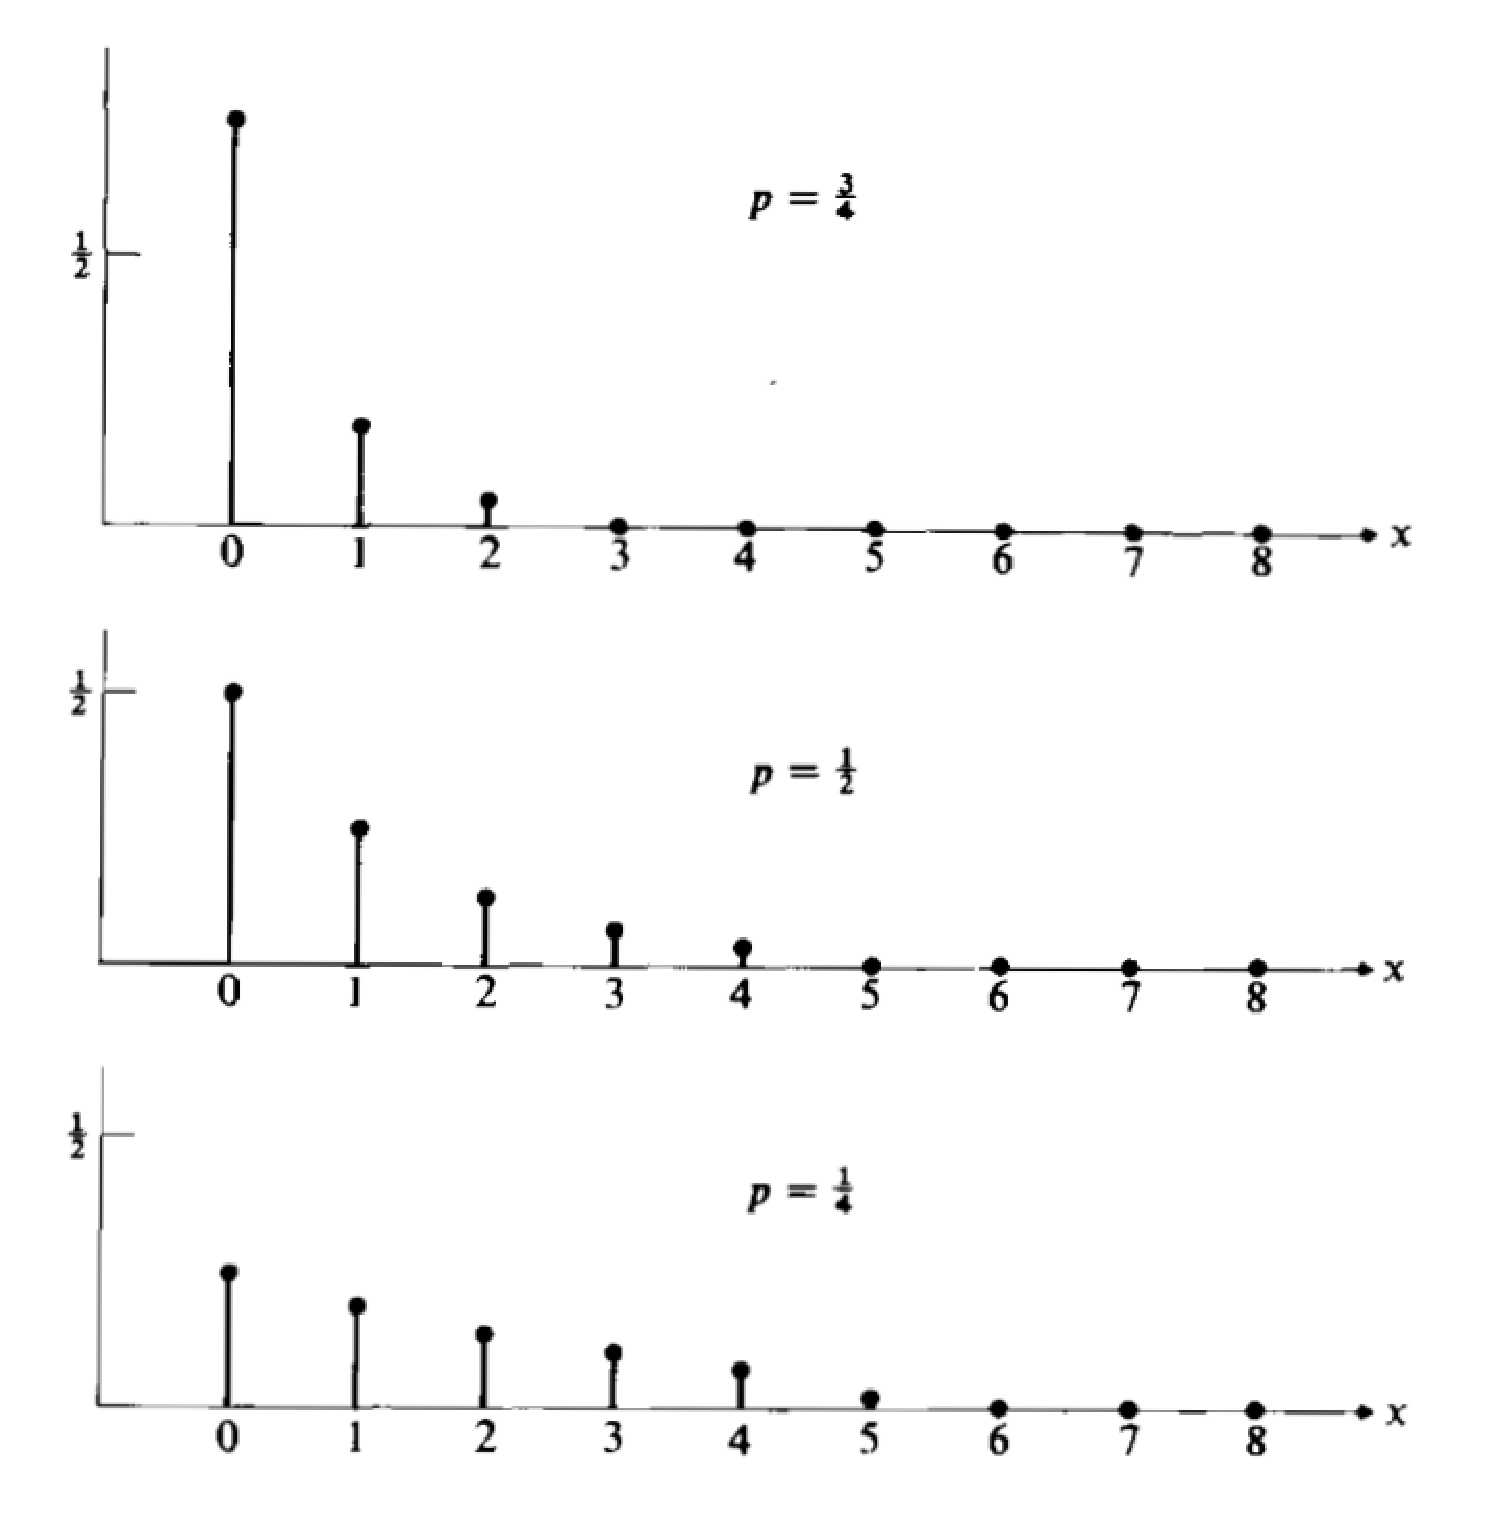
\includegraphics[scale = 0.3]{pictures/geometric_distribution.eps}
\caption{Pravděpodobnostní funkce geometrického rozdělení}
\label{geometric_distribution}
\end{figure}

\begin{theorem}
Jestliže náhodná veličina $X$ sleduje geometrické rozdělení, pak
\begin{gather*}
E[X] = \frac{q}{p}\\
D[X] = \frac{q}{p^2}\\
m(t) = \frac{p}{1 - qe^t}
\end{gather*}
\end{theorem}

\begin{proof}
Vzhledem k tomu, že geometrické rozdělení se speciální případ negitivního binomické rozdělení, odkazujeme se na příslušný důkaz pro negativní binomické rozdělení.
\end{proof}

\begin{theorem}
Jestliže náhodná veličina $X$ sleduje geometrické rozdělení, pak
\begin{equation*}
P[X \ge i + j | X \ge i] = P[x \ge j]~~~\textit{pro}~i,j = 0,1,2,...
\end{equation*}
\end{theorem}

\begin{proof}
\begin{gather*}
P[X \ge i + j|X \ge i] = \frac{P[X \ge i + 1]}{P[X \ge i]} = \frac{\sum_{x = i + j}^{\infty}p(1-p)^x}{\sum_{x=i}^{\infty}p(1-p)^x}\\
= \frac{(1 - p)^{i + j}}{(1 + p)^i} = (1-p)^j = P[X \ge j]
\end{gather*}
\end{proof}

\begin{example}
Uvažujme sérii vzájemně nezávislých Bernoulliho pokusů s pravděpodobostní úspěch $p$. Nechť náhodná veličina $X$ představuje počet neúspěšných pokusů, které předchází prvnímu úspěšnému pokusu. Pak sleduje náhodná veličina $X$ geometrické rozdělení.
\end{example}

\subsubsection{Negativní binomické rozdělení}

\begin{definition}[Negativní binomické rozdělení]
Jestliže náhodná veličina $X$ sleduje negativní binomické rozdělení, pak její pravděpodobnostní funkce má tvar
\begin{gather*}
f_X(x) =
\begin{cases}
\binom{r + x -1}{x} p^r q^x = \binom{-r}{x}p^r (-q)^r~~~\textit{pro}~x = 0, 1, 2,...\\
0~~~\textit{v ostatních případech}
\end{cases}\\
= \binom{r + x -1}{x}p^r q^x I_{\{0,1,2,...\}}(x)
\end{gather*}
kde $r = 1, 2, 3, ...$, $0 < p \le 1$ a $q = 1 - p$.
\end{definition}
Jestliže $r = 1$ pak se negativní binomické rozdělení zredukuje na geometrické rozdělení.

\begin{theorem}
Nechť má náhodná veličina $X$ negativní binomické rozdělení. Pak
\begin{gather*}
E[X] = \frac{rq}{p}\\
D[X] = \frac{rq}{p^2}\\
m(t) = \Big[\frac{p}{1 - qe^t} \Big]^r
\end{gather*}
\end{theorem}

\begin{proof}
\begin{gather*}
m(t) = E[e^{tX}] = \sum_{x = 0}^{\infty} e^{tx}\binom{-r}{x}p^r(-q)^x\\
= \sum_{x=0}^{\infty} \binom{-r}{x}p^r(-qe^t)^x = \Big[ \frac{p}{1 - qe^x} \Big]^r
\end{gather*}
kde jsme využili vztah
\begin{equation*}
(1 - x)^{-n} = \sum_{j = 0}^{\infty} \binom{-n}{j}(-x)^j = \sum_{j = 0}^{\infty} \binom{n + j - 1}{j} x^j~~~\textit{pro}~-1 < x < 1
\end{equation*}
Následnou derivací pak získáme
\begin{gather*}
m'(t) = p^r(-r)(1 - qe^t)^{-r-1}(-qe^t)\\
m''(t) = rqp^r \big[q(r+1)e^{2t}(1 - qe^t)^{-r-2} + e^t(1 - qe^t)^{-r-1} \big]
\end{gather*}
a proto
\begin{gather*}
E[X] = m'(t)\Big|_{t = 0} = \frac{rq}{p}\\
D[X] = m''(t)\Big|_{t = 0} - E[X]^2 = rqp^r[qp^{-r-2}(r+1) + p^{-r-1}] - \Big(\frac{rq}{p}\Big)^2\\
= \frac{rq^2}{p^2} + \frac{rq}{p} = \frac{rq}{p^2}
\end{gather*}
\end{proof}

\begin{example}
Uvažujme sérii vzájemně nezávislých Bernoulliho pokusů s pravděpodobností úspěchu $p$. Nechť náhodná veličina $X$ představuje počet neúspěšných pokusů, které předcházely $r$-tému úspěšnému pokusu. V tomto případě sleduje náhodná veličina $X$ negativní binomické rozdělení.

Odvození pravděpodobnostní funkce je následující. Poslední pokus musí skončit úspěchem. Mezi zbývajícími $x + r - 1$ pokusy musí být $x$ neúspěchů a $r - 1$ úspěchů, přičemž na jejich pořadí nezáleží. Výsledná pravděpodobnost je tak rovna
\begin{equation*}
\binom{x + r - 1}{r - 1}p^{r-1}q^x = \binom{r + x - 1}{x}p^{r-1}q^x
\end{equation*}
\end{example}

\subsection{Ostaní nespojitá rozdělení}

\subsubsection{Odvození ze stávajících rozdělení}

Jedním ze způsobů, jak vytvořit nová nespojitá rozdělení z výše uvedených, je pomocí ``seříznutí''. Pro ilustraci uvažujme Poissonovo rozdělení ``seříznuté'' v bodě 0. V některých situacích nemůže náhodná veličina nabývat hodnoty nula, avšak přesto se Poissonovo rozdělení zdá být vhodným modelem. Odpovídající pravděpodobnostní funkce pak má tvar
\begin{equation*}
f(x) =
\begin{cases}
\frac{e^{-\lambda} \lambda^x}{x!}\big(1 - e^{-\lambda} \big)~~~\textit{pro}~x = 1, 2, 3, ...\\
0~~~\textit{v ostatních případech}
\end{cases}
\end{equation*}
O takto odvozených pravděpodobnostních rozděleních hovoříme jako o zredukovaných pravděpodobnostních rozděleních.

Další způsob odvození nového typu nespojitého rozdělení opět ilustrujme na Poissonově rozdělení. Předpokládejme, že náhodná veličina $X$ sleduje Poissonovo rozdělení. Dále předpokládejme, že v rámci experimentu jsme, z určitých blíže nespecifikovaných důvodů, schopni rozlišit pouze žádnou, jednu nebo více než jednu realizaci. V tomto případě má pravděpodobnostní funkce tvar
\begin{equation*}
f(x) =
\begin{cases}
e^{-\lambda}~~~\textit{pro}~ x = 0\\
\lambda e^{-\lambda}~~~\textit{pro}~ x = 1\\
1 - e^{-\lambda} - \lambda e^{-\lambda}
\end{cases}
\end{equation*}
O náhodné velčině $X$ pak hovoříme jako o censorované náhodné veličině.

\subsubsection{Beta-binomické rozdělení}

\begin{definition}[Beta-binomické rozdělení]
Jestliže náhodná veličina $X$ sleduje beta-binomické rozdělení, pak její pravděpodobnostní funkce má tvar
\begin{equation*}
f(x) = \binom{n}{x} \frac{\Gamma(\alpha + \beta)}{\Gamma(\alpha) \Gamma(\beta)}\frac{\Gamma(x + \alpha) \Gamma(n + \beta - x)}{\Gamma(n + \alpha + \beta)}I_{\{0,1,...,n\}}(x)
\end{equation*}
kde $n$ je přirozené číslo větší než nula, $\alpha > 0$, $\beta > 0$ a $\Gamma(m)$ kde je tzv. gamma funkce
\begin{equation*}
\Gamma(m) = \int_0^{\infty}X^{m-1}e^{-x}dx,~~~ m > 0
\end{equation*}
Pro tuto náhodnou veličinu pak platí
\begin{gather*}
E[X] = \frac{n \alpha}{\alpha + \beta}\\
D[X] = \frac{n \alpha \beta (n + \alpha + \beta)}{(\alpha + \beta)^2(\alpha + \beta + 1)}
\end{gather*}
\end{definition}
Jestliže $\alpha = \beta = 1$, pak se beta-binomické rozdělení zredukuje na nespojité uniformní rozdělení.

\begin{definition}[Logaritmické rozdělení]
Jestliže náhodná veličina $X$ sleduje logaritmické rozdělení, pak její pravděpodobnostní funkce má tvar
\begin{gather*}
f(x) =
\begin{cases}
\frac{q^x}{-x \ln(p)}~~~\textit{pro}~x = 1, 2, ...\\
0~~~\textit{v ostatních případech}
\end{cases}\\
= \frac{q^x}{-x \ln(p)}I_{\{1, 2, ...\}}(x)
\end{gather*}
Pro tuto náhodnou veličinu pak platí
\begin{gather*}
E[X] = \frac{q}{-p \ln(p)}\\
D[X] = \frac{q(q + \ln(p))}{-\big(p \ln(p) \big)^2}
\end{gather*}
\end{definition}
Označení ``logaritmické rozdělení'' vychází ze skutečnosti, že odpovídající pravděpodobnostní funkce je rozvojem $\ln(1 - q)$. Logaritmické rozdělení lze odvodit jako limitní rozdělení negativního binomického rozdělení zobecněného pomocí parametru $r$, který představuje libovolné kladné číslo (nejen celé kladné číslo), a které je seříznuté v bodě 0.

\section{Spojité pravděpodobnostní rozdělení}

\subsection{Spojité uniformní rozdělení}

\begin{definition}[Spojité uniformní rozdělení]
Jestliže náhodná veličina $X$ sleduje spojité uniformní rozdělení, pak její pravděpodobnostní funkce má tvar
\begin{equation*}
f(x) = \frac{1}{b - a}I_{[a, b]}(x)
\end{equation*}
kde $-\infty < a < b < \infty$.
\end{definition}

\begin{figure}[htp]
\centering
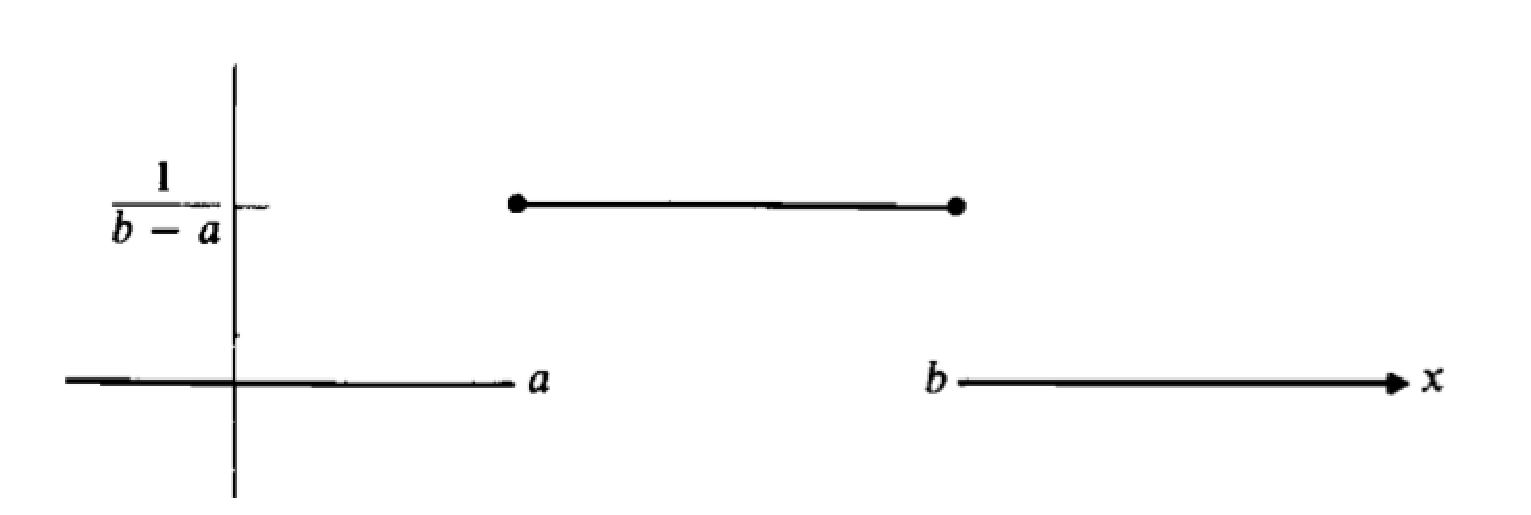
\includegraphics[scale = 0.5]{pictures/continuous_uniform_distribution.eps}
\caption{Pravděpodobnostní funkce spojitého uniformního rozdělení}
\label{continuous_uniform_distribution}
\end{figure}

\begin{theorem}
Jestliže má náhodná veličina $X$ spojité uniformní rozdělení, pak
\begin{gather*}
E[X] = \frac{a + b}{2}\\
D[X] = \frac{(b - a)^2}{12}\\
m(t) = \frac{e^{bt} - e^{at}}{(b - a)t}
\end{gather*}
\end{theorem}

\begin{proof}
\begin{gather*}
E[X] = \int_a^b x \frac{1}{b - a}dx = \frac{b^2 - a^2}{2(b - a)} = \frac{a + b}{2}\\
D[X] = E[X^2] - E[X]^2 = \int_a^b x^2 \frac{1}{b - a}dx - \Big(\frac{a + b}{2}\Big)^2\\
= \frac{b^3 - a^3}{3(b - a)} - \frac{(a + b)^2}{4} = \frac{(b - a)^2}{12}\\
m(t) = E[e^{tX}] = \int_a^b e^{tx} \frac{1}{b - a}dx = \frac{e^{bt} - e^{at}}{(b - a)t}
\end{gather*}
\end{proof}

\begin{theorem}
Kumulativní distribuční funkce spojitého uniformního rozdělení je
\begin{equation*}
F(x) = \frac{x - a}{b - a}I_{[a,b]}(x) + I_{(b, \infty)}(x)
\end{equation*}
\end{theorem}

Ačkoliv jsme definovali uniformní rozdělení nad uzavřeným intervalem $[a, b]$, lze toto rozdělení definovat nad intervalem $(a, b)$, $[a, b)$ nebo $(a,b]$. Pravděpodobnostní funkce bychom modifikovali do podoby $f(x) = \frac{1}{b - a}I_{(a, b)}(x)$, $f(x) = \frac{1}{b - a}I_{[a, b)}(x)$ resp. $f(x) = \frac{1}{b - a}I_{(a, b]}(x)$. Kumulativní distribuční funkce je však ve všech případech shodná.

\subsection{Normální rozdělení}

\begin{definition}[Normální rozdělení]
Jestliže náhodná veličina $X$ sleduje normální rozdělení, pak má její pravděpodobnostní funkce tvar
\begin{equation*}
f(x) = \frac{1}{\sqrt{2 \pi \sigma}} e^{-\frac{(x - \mu)^2}{2 \sigma^2}}
\end{equation*}
kde $-\infty < \mu < \infty$ a $\sigma > 0$. Jak ukážeme později, tyto parametry představuje střední hodnotu a směrodatnou odchylku tohoto pravděpodobnostního rozdělení.
\end{definition}

\begin{figure}[htp]
\centering
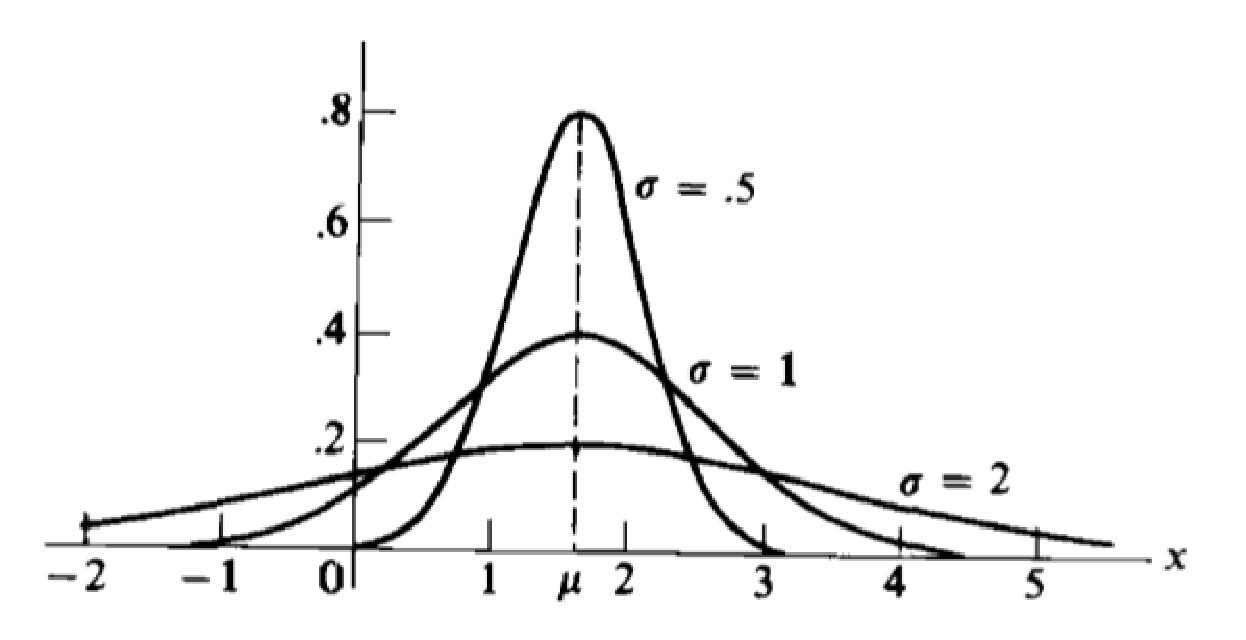
\includegraphics[scale = 0.5]{pictures/normal_distribution.eps}
\caption{Pravděpodobnostní funkce normálního rozdělení}
\label{normal_distribution}
\end{figure}

\begin{figure}[htp]
\centering
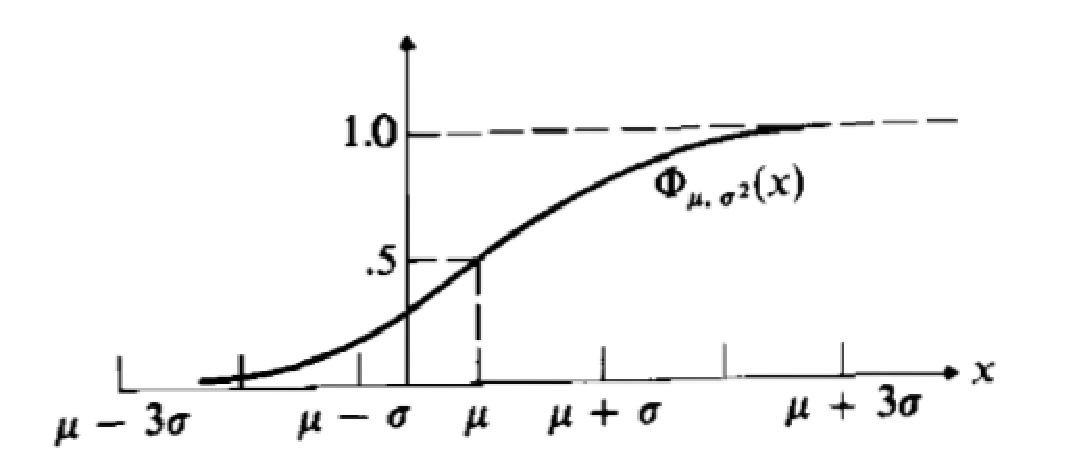
\includegraphics[scale = 0.5]{pictures/normal_cumulative_distribution.eps}
\caption{Kumulativní distribuční funkce normálního rozdělení}
\label{normal_cumulative_distribution}
\end{figure}   

Vzhledem k tomu, že normální rozdělení je velmi často používané, je pro jeho pravděpodobnostní funkci resp. kumulativní distribuční funkci používáno označení $\phi(\mu, \sigma^2)$ resp. $\Phi(\mu, \sigma^2)$. Jestliže $\mu = 0$ a $\sigma = 0$, hovoříme o tzv. standardizovaném popř. normalizovaném normálním rozdělení. V tomto případě se obvykle parametery v značení pravděpodobnostní a kumulativní distribuční funkce vypouštějí.

Protože je $\phi(\mu, \sigma^2)$ pravděpodobnostní funkcí, musí platit
\begin{equation*}
\int_{-\infty}^{\infty} \phi(\mu, \sigma^2)(x) dx = 1
\end{equation*}

\begin{proof}
Uvažujme neurčitý integrál
\begin{equation*}
A = \frac{1}{\sqrt{2 \pi} \sigma} \int_{-\infty}^{\infty} e^{-\frac{(x - \mu)^2}{2 \sigma^2}}dx
\end{equation*}
který lze s využitím substituce $y = \frac{x - \mu}{\sigma}$ upravit do tvaru
\begin{equation*}
A = \frac{1}{\sqrt{2 \pi}} \int_{-\infty}^{\infty} e^{-\frac{1}{2}y^2}dy
\end{equation*}
Potřebuje dokázat $A = 1$. Vzhledem k tomu, že $e^t$ je kladné pro všechna $t$, platí $A > 0$. Pokud bychom dokázali $A^2 = 1$, pak by to implikovalo $A = 1$. $A^2$ lze vyjádřit jako
\begin{gather*}
A^2 = \frac{1}{\sqrt{2 \pi}} \int_{-\infty}^{\infty} e^{-\frac{1}{2}y^2}dy \frac{1}{\sqrt{2 \pi}} \int_{-\infty}^{\infty} e^{-\frac{1}{2}z^2}dz\\
= \frac{1}{2 \pi} \int_{-\infty}^{\infty} \int_{-\infty}^{\infty} e^{-\frac{1}{2}(y^2 + z^2)}dydz
\end{gather*}
Následně tento integrál převedeme pomocí substitucí $y = r \sin(\theta)$ a $z = r \cos(\theta)$ do polárních souřadnic.
\begin{equation*}
A^2 = \frac{1}{2 \pi} \int_0^{\infty} \int_0^{2 \pi} r e^{-\frac{1}{2} r^2}d \theta dr = \int_0^{\infty} = r e^{-\frac{1}{2}r^2}dr = 1
\end{equation*}
\end{proof}

\begin{theorem}
Jestliže náhodná veličina $X$ sleduje normální rozdělení, pak
\begin{gather*}
E[X] = \mu\\
D[X] = \sigma^2\\
m(t) = e^{\mu + \sigma^2 t^2 / 2}
\end{gather*}
\end{theorem}
\begin{proof}
\begin{gather*}
m(t) = E[e^{tX}] = e^{t \mu}E[e^{t(X-\mu)}] = e^{t \mu} \int_{-\infty}^{\infty} \frac{1}{\sqrt{2 \pi}} e^{t(x-\mu)}e^{-(1/2\sigma^2)(x-\mu)^2}dx\\
= e^{t\mu} \frac{1}{\sqrt{2 \pi}} \int_{-\infty}^{\infty} e^{-(1/2 \sigma^2)[(x - \mu)^2 - 2 \sigma^2 t(x - \mu)]}dx
\end{gather*}
Jestliže doplníme kvadráty v závorkách
\begin{gather*}
(x - \mu)^2 - 2 \sigma^2 t(x - \mu) = (x - \mu)^2 - 2 \sigma^2 t(x - \mu) + \sigma^4 t^2 - \sigma^4 t^2\\
=(x - \mu - \sigma^2 t)^2 - \sigma^4 t^2
\end{gather*}
získáme
\begin{equation*}
m(t) = e^{t \mu} e^{\sigma^2 t^2 / 2} \frac{1}{\sqrt{2 \pi} \sigma} \int_{-\infty}^{\infty} e^{-(x - \mu - \sigma^2 t)^2 / 2 \sigma^2}dx
\end{equation*}
Integrál společně s členem $\frac{1}{\sqrt{2 \pi} \sigma}$ musí být roven 1, protože se jedná o plochu pod pravděpodobnostní funkcí normálního rozdělení se střední hodnotou $\mu + \sigma^2 t$ a rozptylem $\sigma^2$, a proto
\begin{equation*}
m(t) = e^{\mu t + \sigma^2 t^2 / 2}
\end{equation*}
Derivací $m(t)$ pro $t = 0$ získáme
\begin{gather*}
E[X] = m'(0) = \mu\\
D[X] = E[X^2] - E[X]^2 = m''(0) - \mu^2 = \sigma^2
\end{gather*}
\end{proof}

\begin{theorem}
Protože neurčitý integrál $\sigma_{\mu, sigma^2}(x)$ nelze řešit analyticky, jsme schopni kumulativní distribuční funkci prezentovat pouze ve tvaru
\begin{equation*}
\Phi_{\mu, \sigma^2}(x) = \int_{-\infty}^x \phi_{\mu, \sigma^2}(u)du
\end{equation*}
\end{theorem}
\begin{theorem}
Jestliže má náhodná veličina $X$ normální rozdělení, pak
\begin{equation*}
P[a < X < b] = \Phi \Big(\frac{b - \mu}{\sigma}\Big) - \Phi \Big(\frac{a - \mu}{\sigma}\Big)
\end{equation*}
\end{theorem}
\begin{proof}
\begin{gather*}
P[a < X < b] = \int_a^b \frac{1}{\sqrt{2 \pi} \sigma} e^{-\frac{1}{2}[(x - \mu)/\sigma]^2}dx\\
= \int_{(a - \mu)/\sigma}^{(b - \mu)/\sigma} \frac{1}{\sqrt{2 \pi}} e^{-\frac{1}{2}z^2}dz\\
= \Phi \Big(\frac{b - \mu}{\sigma}\Big) - \Phi \Big(\frac{a - \mu}{\sigma}\Big)
\end{gather*}
\end{proof}

\begin{theorem}
Velmi užitečným vztahem je
\begin{equation*}
\Phi(x) = 1 - \Phi(-x)
\end{equation*}
což vyplývá ze symetričnosti normálního rozdělení.
\end{theorem}

\begin{example}
Předpokládejme, že průměr strojově vyráběné kovové tyče má normální rozdělení se střední hodnotou 10 cm a směrodatnou odchylkou 0.1 cm. Aby mohla být tyč použita v navazující výrobě, musí být její průměr v rozmezí 9.9 až 10.2 cm. Jaké procento vyrobených tyčí splňuje tuto podmínku?

\begin{gather*}
P[9.9 < X < 10.2] = \Phi \Big(\frac{10.2 - 10}{0.1} \Big) - \Phi \Big(\frac{9.9 - 10}{0.1} \Big)\\
= \Phi(2) - \Phi(-1) \approx 0.9772 - 0.1587 = 0.8185
\end{gather*}
\end{example}

\subsection{Exponenciální a gamma rozdělení}

\subsubsection{Exponenciální rozdělení}

\begin{definition}[Exponenciální rozdělení]
Jestliže náhodná veličina $X$ sleduje exponenciální rozdělení, pak má její pravděpodobnostní funkce tvar
\begin{equation*}
f(x) = \lambda e^{- \lambda x}I_{[0, \infty)}(x)
\end{equation*}
kde $\lambda > 0$.
\end{definition}
\begin{theorem}
Jestliže náhodná veličina $X$ sleduje exponenciální rozdělení, pak
\begin{gather*}
E[X] = \frac{1}{\lambda}\\
D[X] = \frac{1}{\lambda^2}\\
m(t) = \frac{\lambda}{\lambda - t}
\end{gather*}
\end{theorem}

\begin{proof}
Vzhledem k tomu, že exponenciální rozdělení je specifickým případem gamma rozdělení, odkazujeme se na příslušný důkaz pro toto rozdělení.
\end{proof}

Jestliže lze v rámci určitého experimentu modelovat počet realizací za časovou jednotku pomocí Poissonova rozdělení, pak lze délku trvání jednotlivých realizací modelovat pomocí exponenciálního rozdělení.

\begin{theorem}
Jestliže náhodná veličina $X$ sleduje exponenciální rozdělení, pak
\begin{equation*}
P[x > a + b| X > a] = P[X > b]~~~\textit{pro}~a > 0 ~\textit{a}~ b > 0
\end{equation*}
\end{theorem}
\begin{proof}
\begin{equation*}
P[X > a + b | X > a] = \frac{P[X > a + b]}{P[X > a]} = \frac{e^{-\lambda(a + b)}}{e^{-\lambda a}} = e^{-\lambda b} = P[X > b]
\end{equation*}
\end{proof}

\subsubsection{Gamma distribuce}

\begin{definition}[Gamma rozdělení]
Jestliže náhodná veličina $X$ sleduje gamma rozdělení, pak má její pravděpodobnostní funkce tvar
\begin{equation*}
f(x) = \frac{\lambda}{\Gamma(r)}(\lambda x)^{r - 1}e^{-\lambda x}I_{[0, \infty)}(x)
\end{equation*}
kde $r > 0$, $\lambda > 0$ a $\Gamma(\cdot)$ je tzv. gamma funkce.
\end{definition}
Jestliže je parametr $r$ roven jedné, pak se gamma distribuce zredukuje na exponenciální rozdělení.

\begin{figure}[htp]
\centering
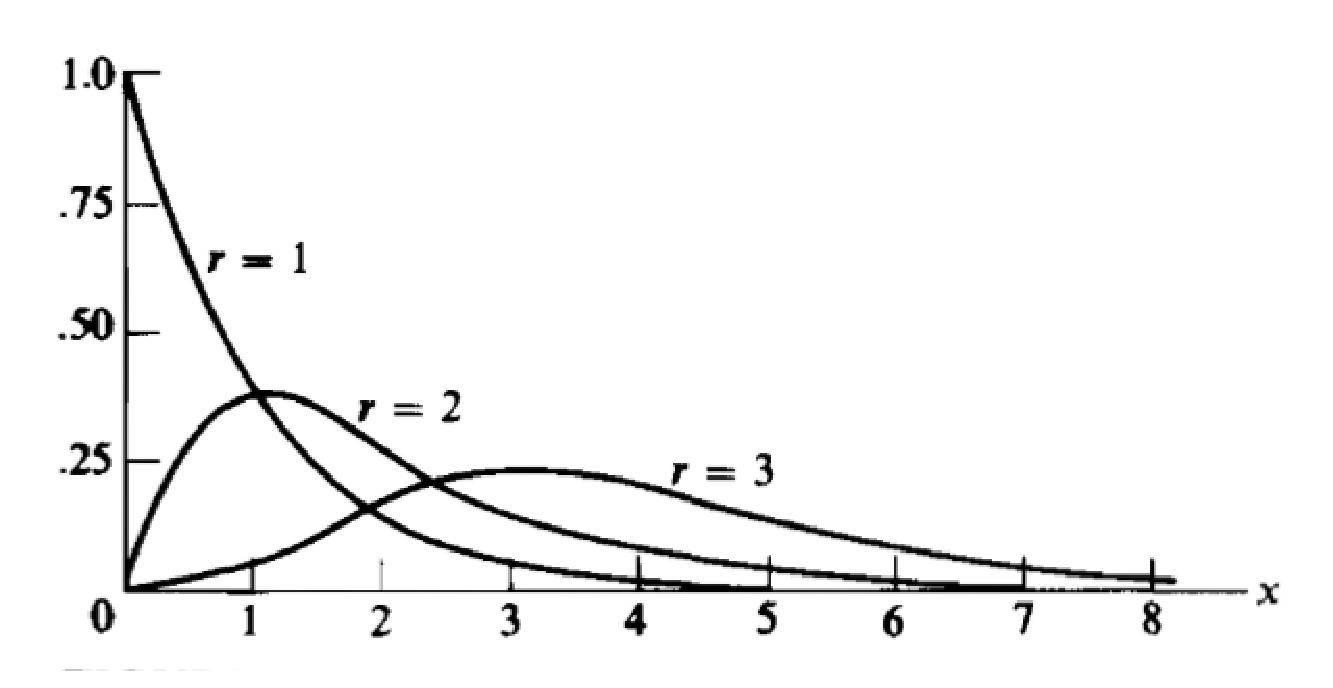
\includegraphics[scale = 0.5]{pictures/gamma_distribution.eps}
\caption{Pravděpodobnostní funkce gamma rozdělení}
\label{gamma_distribution}
\end{figure}

\begin{theorem}
Jestliže náhodná veličina $X$ sleduje gamma rozdělení, pak
\begin{gather*}
E[X] = \frac{r}{\lambda}\\
D[X] = \frac{r}{\lambda^2}\\
m(t) = \Big(\frac{\lambda}{\lambda - t} \Big)^r~~~\textit{pro}~t < \lambda
\end{gather*}
\end{theorem}
\begin{proof}
\begin{gather*}
m(t) = E[e^{tX}] = \int_0^{\infty} \frac{\lambda^r}{\Gamma(r)}e^{tx}x^{r-1}e^{-\lambda x} dx\\
= \Big(\frac{\lambda}{\lambda - t} \Big)^r \int_0^{\infty} \frac{(\lambda - t)^r}{\Gamma(r)}x^{r-1}e^{-(\lambda - t)x}dx = \Big( \frac{\lambda}{\lambda - t} \Big)^r
\end{gather*}
První a druhá derivace momentové funkce jsou pak
\begin{gather*}
m'(t) = r \lambda^r (\lambda - t)^{-r - 1}\\
m''(t) = r(r + 1)\lambda^r(\lambda - t)^{-r-2}
\end{gather*}
a proto
\begin{gather*}
E[X] = m'(0) = \frac{r}{\lambda}\\
D[X] = E[X^2] - E[X]^2 = m''(0) - \Big(\frac{r}{\lambda}\Big)^2 = \frac{r(r+1)}{\lambda^2} - \Big(\frac{r}{\lambda}\Big)^2 = \frac{r}{\lambda^2}
\end{gather*}
\end{proof}

Jestliže lze počet realizací v rámci určitého experimentu modelovat pomocí Poissonova rozdělení, pak lze délku časového úseku od okamžiku 0 do okamžiku $r$-té realizace modelovat pomocí gamma distribuce. Jedná se tedy o čas, který musíme čekat, než dojde k $r$-té realizaci.

\begin{theorem}
Jestliže náhodná veličina $X$ sleduje gamma rozdělení, kde parametr $r$ je kladné celé číslo, pak
\begin{equation*}
F(x) = 1 - \sum_{j = 0}^{r-1}\frac{e^{\lambda x}(\lambda x)^j}{j!}
\end{equation*}
\end{theorem}
\begin{proof}
Výše uvedenou větu lze dokázat postupným integrováním per partes.
\end{proof}

\subsection{Beta rozdělení}

\begin{definition}[Beta rozdělení]
Jestliže náhodná veličina $X$ sleduje beta rozdělení, pak její pravděpodobnostní funkce má tvar
\begin{equation*}
f(x) = \frac{1}{B(a,b)}x^{n-1}(1 - x)^{b - 1}I_{(0,1)}(x)
\end{equation*}
kde $a > 0$, $b > 0$ a $B(a, b) = \int_0^1 x^{a - 1}(a1 - x)^{b - 1}dx$ je tzv. beta funkce.
\end{definition}

Pro $a = b$ se beta rozdělení zredukuje na spojité uniformní rozdělení nad intervalem $(0, 1)$.

\begin{figure}[htp]
\centering
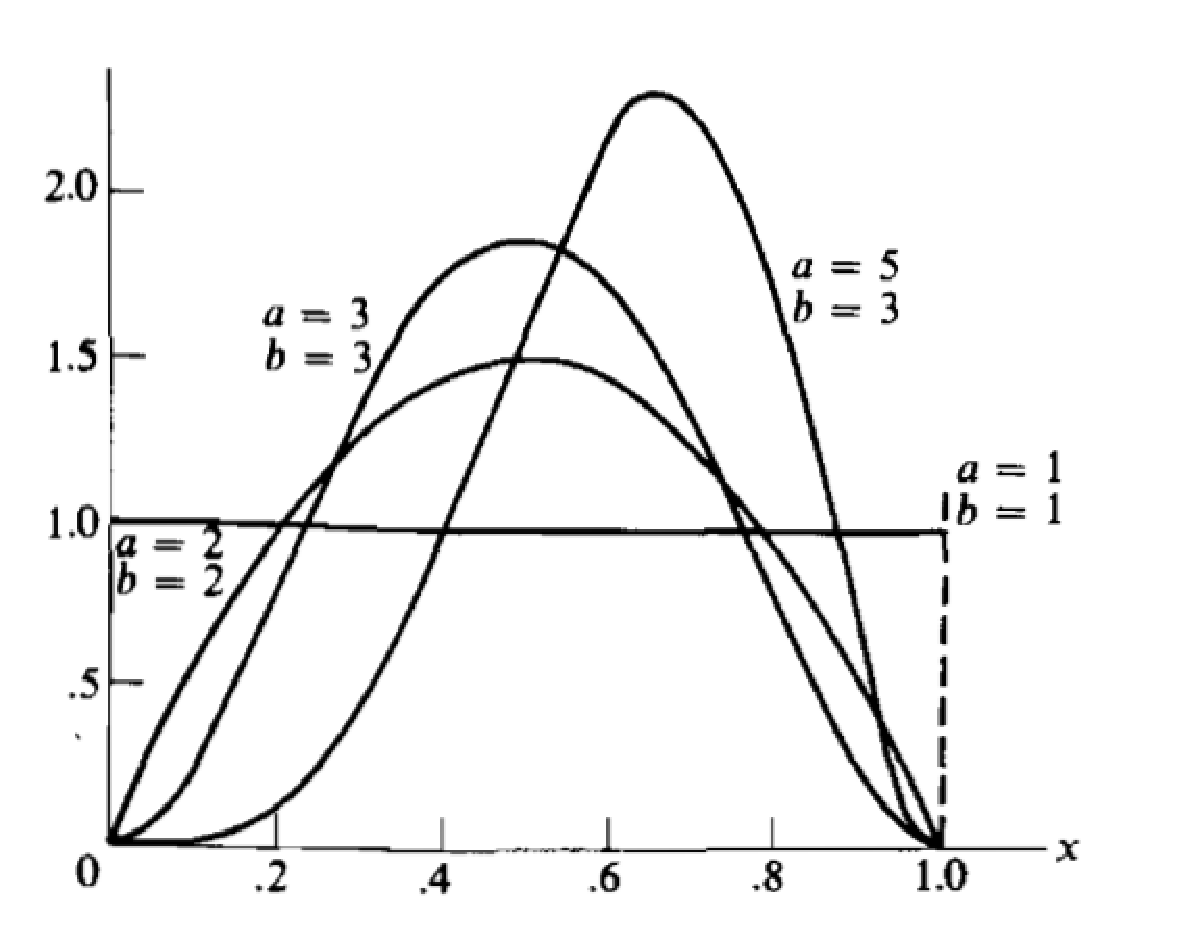
\includegraphics[scale = 0.5]{pictures/beta_distribution.eps}
\caption{Pravděpodobnostní funkce beta rozdělení}
\label{beta_distribution}
\end{figure}

\begin{theorem}
Kumulativní distribuční funkce náhodné veličiny $X$ s beta rozdělením má tvar
\begin{equation*}
F(x) = I_{(0, 1)}(x) \int_0^x \frac{1}{B(a, b)}u^{a - 1}(1 - u)^{b - 1}du + I_{[1, \infty)}(x)
\end{equation*}
\end{theorem}

Momentová funkce beta rozdělení nemá jednoduchou analytickou formu, nicméně momenty lze snadno odvodit přímo z jejich definice, tj. bez použití momentové funkce.

\begin{theorem}
\begin{gather*}
E[X] = \frac{a}{a + b}\\
D[X] = \frac{ab}{(a + b + 1)(a + b)^2}
\end{gather*}
\end{theorem}
\begin{proof}
\begin{gather*}
E[X^k] = \frac{1}{B(a, b)} \int_0^1 x^{k + a - 1}(1 - x)^{b - 1}dx\\
=\frac{B(k + a, b)}{B(a, b)} = \frac{\Gamma(k + a)\Gamma(b)}{\Gamma(k + a + b)} \frac{\Gamma(a + b)}{\Gamma(a) \Gamma(b)}\\
= \frac{\Gamma(k + a)\Gamma(a + b)}{\Gamma(a) \Gamma(k + a + b)}
\end{gather*}
Proto
\begin{gather*}
E[X] = \frac{\Gamma(a + 1) \Gamma(a + b)}{\Gamma(a) \Gamma(a + b + 1)} = \frac{a}{a + b}\\
D[X] = E[X^2] - E[X]^2 = \frac{\Gamma(a + 2)\Gamma(a + b)}{\Gamma(a) \Gamma(a + b + 2)} - \Big(\frac{a}{a + b}\Big)^2\\
= \frac{(a + 1)a}{(a + b + 1)(a + b)} - \Big(\frac{a}{a + b}\Big)^2 = \frac{ab}{(a + b + 1)(a + b)^2}
\end{gather*}
\end{proof}

Beta rozdělení nabývá na intervalu $(0, 1)$ kladných hodnot a její pravděpodobnostní funkce je charakteristická velkým množstvím tvarů.

\section{Ostatní spojitá rozdělení}

V této kapitole budou představena některá další spojitá rozdělení. Studentovo, chi-kvadrát a F rozdělení budou představena později.

\subsection{Cauchyho rozdělení}

\begin{definition}[Cauchyho rozdělení]
Jestliže náhodná veličina $X$ sleduje Cauchyho rozdělení, pak její pravděpodobnostní funkce má tvar
\begin{equation*}
f(x) = \frac{1}{\pi \beta \big(1 + \big(\frac{x - a}{\beta} \big)^2 \big)}
\end{equation*}
kde $-\infty < \alpha < \infty$ a $\beta > 0$.
\end{definition}
Cauchyho rozdělení je symetrické okolo parametru $\alpha$, avšak střední hodna a vyšší momenty nejsou definovány.

\begin{theorem}
Kumulativní distribuční funkce Cauchyho rozdělení má tvar
\begin{gather*}
F(x) = \frac{1}{\pi} \int_{-\infty}^x \frac{1}{\pi \beta \big(1 + \big(\frac{u - a}{\beta}\big)^2 \big)}du\\
= \frac{1}{2} + \frac{1}{\pi}arctan \Big( \frac{x - \alpha}{\beta}\Big)
\end{gather*}
\end{theorem}

\subsection{Lognormální rozdělení}

\begin{definition}[Lognormální rozdělení]
Nechť je $X$ kladná náhodná veličina a definujme novou náhodnou veličinu $Y = \ln(X)$. Sleduje-li $Y$ normální rozdělení, pak sleduje $X$ lognormální rozdělení. Pravděpodobnostní funkce lognormálního rozdělení má tvar
\begin{equation*}
f(x) = \frac{1}{x \sqrt{2 \pi} \sigma}e^{-\frac{1}{2 \sigma^2}(\ln(x) - \mu)^2}I_{(0, \infty)}(x)
\end{equation*}
kde $-\infty < \mu < \infty$ a $\sigma > 0$.
\end{definition}

\begin{theorem}
Jestliže náhodná veličina $X$ sleduje lognormální rozdělení, pak
\begin{gather*}
E[X] = e^{\mu + \frac{1}{2}\sigma^2}\\
D[X] = e^{2 \mu + 2 \sigma^2} - e^{2\mu + \sigma^2}
\end{gather*}
\end{theorem}

Jestliže má $X$ lognormální rozdělení, pak $E[\ln(X)] = \mu$ a $D[\ln(X)] = \sigma^2$.

\subsection{Laplaceova distribuce}

\begin{definition}[Laplaceova distribuce]
Jestliže náhodná veličina $X$ sleduje Laplaceovo rozdělení, pak má její pravděpodobnostní funkce tvar
\begin{equation*}
f(x) = \frac{1}{2 \beta} e^{-\frac{|x - \alpha|}{\beta}}
\end{equation*}
kde $-\infty < \alpha < \infty$ a $\beta > 0$.
\end{definition}

\begin{theorem}
Jestliže náhodná veličina $X$ sleduje Laplaceovo rozdělení, pak
\begin{gather*}
E[X] = \alpha\\
D[X] = 2 \beta^2
\end{gather*}
\end{theorem}

\subsection{Weibullovo rozdělení}

\begin{definition}
Jestliže náhodná veličina $X$ sleduje Weibullovo rozdělení, pak její pravděpodobnostní funkce má tvar
\begin{equation*}
f(x) = abx^{b-1}e^{-ax^b}I_{(0, \infty)}(x)
\end{equation*}
kde $a > 0$ a $b > 0$.
\end{definition}

\begin{theorem}
Jestliže náhodná veličina $X$ sleduje Weibullovo rozdělení, pak
\begin{gather*}
E[X] = \frac{1}{a}^{\frac{1}{b}}\Gamma(1 + b^{-1})\\
D[X] = \frac{1}{a}^{\frac{2}{b}}\big(\Gamma(1 + 2 b^{-1}) - \Gamma^2(1 + b^{-1}) \big)
\end{gather*}
\end{theorem}

Pro $b = 1$ se Weibullovo rozdělení zredukuje na exponenciální rozdělení.

\subsection{Logistické rozdělení}

\begin{definition}[Logistické rozdělení]
Jestliže náhodná veličina $X$ sleduje logistické rozdělení, pak má její kumulativní distribuční funkce tvar
\begin{equation*}
F(x) = \frac{1}{1 + e^{- \frac{x - \alpha}{\beta}}}
\end{equation*}
kde $-\infty < \alpha < \infty$ a $\beta > 0$.
\end{definition}

\begin{theorem}
Jestliže náhodná veličina $X$ sleduje logistické rozdělení, pak
\begin{gather*}
E[X] =  \alpha\\
D[X] = \frac{\beta^2 \pi^2}{3}
\end{gather*}
\end{theorem}

Pro kumulativní distribuční funkci logistického rozdělení platí $F(\alpha - d) = 1 - F(\alpha + d)$, a pravděpodobnostní funkce je tak symetrická kolem parametru $\alpha$.

\subsection{Paretovo rozdělení}

\begin{definition}[Pareto rozdělení]
Jestliže náhodná veličina $X$ sleduje Paretovo rozdělení, pak má její pravděpodobnostní funkce tvar
\begin{equation*}
f(x) = \frac{\theta}{x_0} \Big(\frac{x_0}{x}\Big)^{\theta + 1}I_{(x_0, \infty)}(x)
\end{equation*}
kde $\theta > 0$ a $x_0 > 0$.
\end{definition}

\begin{theorem}
Jestliže náhodná veličina $X$ sleduje Paretovo rozdělení, pak
\begin{gather*}
E[X] = \frac{\theta x_0}{\theta - 1}~~~ \textit{pro}~ \theta > 0\\
D[X] = \frac{\theta x_0^2}{\theta - 2} - \Big(\frac{\theta x_0}{\theta - 1} \Big)^2 ~~~ \textit{pro}~  > 2
\end{gather*}
\end{theorem}

\section{Poznámky}

\subsection{Aproximace}

Ačkoliv existuje celá řada aproximací jednoho rozdělení pomocí jiného, budeme se v této kapitole zabývat pouze třemi z nich. Některé další aproximace představíme v kapitole o Centrální limitní větě.

\subsubsection{Aproximace binomického rozdělení Poissonovým rozdělením}

Pravděpodobnostní funkce binomického rozdělení má tvar
\begin{equation*}
\binom{n}{x}p^x(1 - p)^{n-x}~~~\textit{pro}~x = 0, 1, ..., n
\end{equation*}
Jestliže se $n$ blíží nekonečnu a $p$ se blíží nule, přičemž $np = \lambda$ zůstává konstantní, pak
\begin{equation*}
\binom{n}{x}p^x(1 - p)^{n-x} \rightarrow \frac{e^{-\lambda} \lambda^x}{x!}
\end{equation*}
pro fixní celé číslo $x$. Výše uvedený vztah vyplývá z
\begin{gather*}
\binom{n}{x}p^x(1 - p)^{n - x} = \frac{(n)_x}{x!}\Big(\frac{\lambda}{n}\Big)^x \Big(1 - \frac{\lambda}{n} \Big)^{n-x}\\
= \frac{\lambda^x}{x!} \frac{(n)_x}{n^x}\Big(1 - \frac{\lambda}{n}\Big)^n\Big(1 - \frac{\lambda}{n} \Big)^{-x} \rightarrow \frac{e^{-\lambda}\lambda^x}{x!}
\end{gather*}
protože
\begin{gather*}
\lim_{n \rightarrow \infty}\frac{(n)_x}{n^x} = 1\\
\lim_{n \rightarrow \infty}\Big(1 - \frac{\lambda}{n}\Big)^{-x} = 1\\
\lim_{n \rightarrow \infty}\Big(1 - \frac{\lambda}{n} \Big)^n = e^{-\lambda}
\end{gather*}
Proto pro dostatečně velká $n$ a malá $p$ lze tedy binomickou pravděpodobnost $\binom{n}{x}p^x(1 - p)^{n-x}$ aproximovat pomocí Poissonovy pravděpodobnosti $\frac{e^{-np}(np)^x}{x!}$.

\subsubsection{Aproximace binomického a Poissonova rozdělení normálním rozdělením}

\begin{theorem}
Nechť náhodná veličina $X$ sleduje Poissonovo rozdělení. Pak pro fixní $a < b$ platí
\begin{equation*}
P\Big[a < \frac{X - \lambda}{\sqrt{\lambda}}\Big] = P[\lambda + a\sqrt{\lambda} < X < \lambda + b\sqrt{\lambda}] \rightarrow \Phi(b) - \Phi(b) ~~~\textit{pro}~ \lambda \rightarrow \infty
\end{equation*}
\end{theorem}

\begin{theorem}[De Moivre-Laplaceova limitní věta]
Nechť náhodná veličina $X$ sleduje binomické rozdělení. Pak pro fixní $a < b$ platí
\begin{equation*}
P\Big[a \le \frac{X - np}{\sqrt{npq}} \le b \Big] = P[np + a \sqrt{npq} \le X \le np + b \sqrt{npq}] \rightarrow \Phi{b} - \Phi(a) ~~~\textit{pro}~ n \rightarrow \infty
\end{equation*}
\end{theorem}

\begin{example}
Uvažujme hrací kostku, která je vržena 600 krát. Nechť náhodná veličina $X$ představuje počet hodů, při kterých padla šestka. Je zřejmé, že $X$ sleduje binomické rozdělení s $n = 600$ a $p = \frac{1}{6}$ a že $E[X] = 100$. Nalezněte pravděpodobnost $P[90 \le X \le 110]$.

Platí
\begin{equation*}
P[90 \le X \le 110] = \sum_{j = 90}^{110}\binom{600}{j}\Big(\frac{1}{6}\Big)^j \Big(\frac{5}{6}\Big)^{600 - j}
\end{equation*}
S využitím aproximace se lze vyhnout rutinnímu výpočtu.
\begin{gather*}
P[90 \le X \le 110] \approx \Phi\Big(\frac{110 - 100}{\sqrt{\frac{500}{6}}}\Big) - \Phi\Big(\frac{90 - 100}{\sqrt{\frac{500}{6}}}\Big)\\
=\Phi \Big(\sqrt{\frac{6}{5}}\Big) - \Phi \Big(\sqrt{-\frac{6}{5}}\Big) \approx \Phi(1.095) - \Phi(-1.095) \approx 0.726
\end{gather*}
\end{example}

\subsection{Vztah mezi Poissonovým a exponenciálním rozdělením}

V předchozím textu jsme ukázali, že Poissonovo rozdělení je vhodné pro modelování počtu vzájemně nezávislých realizací v čase. Předpokládejme, že k jedné takovéto realizaci došlo, a že předmětem našeho zájmu je délka, po kterou budeme muset čekat, než dojde k další realizaci. Pravděpodobnost
\begin{equation*}
P[X > x] = P[\textit{žádná realizace v časovém intervalu délky x}] = e^{-vx}
\end{equation*}
kde $v$ je střední míra realizace. Proto
\begin{equation*}
F(x) = P[X \le x] = 1 - P[X > x] = 1 - e^{-vx} ~~~\textit{pro}~x > 0
\end{equation*}
což znamená, že $X$ má exponenciální rozdělení. Tento vztah platí také naopak. Lze dokázat, že lze-li dobu mezi vzájemně nezávislými realizacemi modelovat pomocí exponenciálního rozdělení, pak lze počet realizací modelovat pomocí Poissonova rozdělení.

\subsection{Smíšená pravděpodobnostní rozdělení}

Uvažujme pravděpodobnostní funkce $f_0(\cdot), f_1(\cdot), ..., f_n(\cdot)$, které jsou všechny buďto spojité nebo nespojité. Dále uvažujme parametry $p_0, p_1, ..., p_n$ které splňují
\begin{gather*}
p_i \ge 0\\
\sum_{i = 0}^{\infty}p_i = 1
\end{gather*}
Pak $\sum_{i = 0}^{\infty}p_i f_i(x)$ představuje pravděpodobnostní funkcí, která vznikla ``smícháním'' pravděpodobnostních funkcí $f_0(\cdot), f_1(\cdot), ..., f_n(\cdot)$.

\begin{example}
Ilustrujme myšlenku smíšeného pravděpodobnostního rozdělení s pomocí pravděpodobnostních funkcí $f_0(x) = \phi(\mu_0, \sigma_0^2)(x)$ a $f_1(x) = \phi(\mu_1, \sigma_1^2)(x)$. Pak
\begin{gather*}
p_0 \phi(\mu_0, \sigma_0^2)(x) + p_1 \phi(\mu_1, \sigma_1^2)(x)\\
= (1 - p) \frac{1}{\sqrt{2 \pi \sigma_0}}e^{-\frac{1}{2}(\frac{x - \mu_0}{\sigma_0})^2} + p \frac{1}{\sqrt{2 \pi \sigma_1}}e^{-\frac{1}{2}(\frac{x - \mu_1}{\sigma_1})^2}
\end{gather*}
\end{example}

Výše uvedené smíšené rozdělení nazýváme smíšeným normálním rozdělením. V našem konkrétním případě má toto rozdělení pět parametrů, což mu umožňuje nabývat nejrůznějších tvarů. Vhodným nastavením parametrů lze tak vytvořit např. bimodální rozdělení, tj. rozdělení se dvěma vrcholy. Díky své flexibilitě je tak ``míchání'' pravděpodobnostních rozdělení často využíváno při modelování některých experimentů.

Koncept smíšeného pravděpodobnostního rozdělení lze dále rozšířit. Nechť $\{f(x; \theta)\}$ představuje rodinu pravděpodobnostních funkcí indexovaných parametrem $\theta$. Množinu všech hodnot, kterých může $\theta$ nabývat, označme $\Theta$. Je-li $\Theta$ interval a $g(\theta)$ pravděpodobnostní funkce, která je nulová pro všechny prvky mimo $\Theta$, pak
\begin{equation*}
\int_{\Theta}f(x; \theta) g(\theta) d\theta
\end{equation*}
je opět pravděpodobnostní funkce.

\begin{example}
Uvažujme $f(x; \theta) = \frac{e^{-\theta}\theta^x}{x!}$ pro $x = 0, 1, 2, ...$ a $f(x; \theta) = 0$ v ostatních případech. Dále uvažujme pravděpodobnostní funkci gamma rozdělení $g(\theta) = \frac{\lambda^r}{\Gamma(r)}\theta^{r-1}e^{-\lambda \theta}I_{(0, \infty)}(\theta)$. Pak
\begin{gather*}
\int_0^{\infty}f(x;\theta)g(\theta)d\theta = \int_0^{\infty} \frac{e^{-\theta}\theta^x}{x!} \frac{\lambda^r}{\Gamma(r)}\theta^{r - 1}e^{-\theta \lambda} d \theta = \frac{\lambda^r}{x! \Gamma(r)} \int_0^{\infty} \theta^{r + x - 1} e^{-(\lambda + 1)\theta}d \theta\\
= \frac{\lambda^r}{x! \Gamma(r)} \frac{\Gamma(r + x)}{(\lambda + 1)^{r + x}}\int_0^{\infty} \frac{[(\lambda + 1)\theta]^{r + x - 1} e^{-(\lambda + 1)\theta}}{\Gamma(r + x)} d[(\lambda + 1)\theta]\\
= \Big(\frac{\lambda}{\lambda + 1}\Big)^r \frac{\Gamma(r + x)}{x!\Gamma(r)}\frac{1}{(\lambda + 1)^x}\\
= \binom{r + x - 1}{x}\Big(\frac{\lambda}{\lambda + 1}\Big)^r\Big(\frac{1}{\lambda + 1}\Big)^x ~~~\textit{pro}~x = 0, 1, 2, ...
\end{gather*}
což je pravděpodobnostní funkce binomického rozdělení s parametery $r$ a $p = \frac{\lambda}{\lambda + 1}$. Na binomické rozdělení je tak možné nahlížet jako na gamma smíšené Poissonovo rozdělení.
\end{example}

\subsection{Zredukovaná pravděpodobnostní rozdělení}

Pro ilustraci uvažujme normální rozdělení ``seříznuté'' zleva hodnotou 0 a zprava hodnotou 1. Pravděpodobnostní funkce takovéhoto zredukovaného pravděpodobnostního rozdělení je
\begin{equation*}
f(x) = \frac{\phi(\mu, \sigma^2)(x)I_{(0,1)}(x)}{\Phi(\mu, \sigma^2)(1) - \Phi(\mu, \sigma^2)(0)}
\end{equation*}

Obecná definice zredukovaného spojitého pravděpodobnostního rozdělení je následující.

\begin{theorem}
Jestliže $X$ je spojitá náhodna veličina s pravděpodobnostní funkcí $f(\cdot)$ a kumulativní distribuční funkcí $F(\cdot)$, pak pravděpodobnostní funkce náhodné veličiny $X$ zredukované na interval $(a, b)$ je
\begin{equation*}
\frac{f(x)I_{(a, b)}(x)}{F(b) - F(a)}
\end{equation*}
\end{theorem}
